\chapter{Preliminaries} \label{chap:preliminaries}

\section{Propositional logic}

Propositional logic serves as the foundational mathematical framework for reasoning over declarative statements using Boolean truth values and formal logical operators. For our purposes, we will be interested in a fragment of propositional logic that works with finite amount of elements. For a more in depth explanation of propositional logic covering topics necessary to understand this work, the reader is referred to \cite{logic_book,kraj_book,galesi_toran}.

Let $\mathrm{Var} = \{x_1, \ldots, x_n\}$ denote a non-empty, finite set of atomic propositional symbols, called \textit{variables}, and let $\mathscr{O} = \{\land, \lor, \lnot, \to, \leftrightarrow\}$ be the set of Boolean logical connectives. Each of these connectives represents, respectively, the concept of conjunction, disjunction, negation, implication and logical equivalence. By recursively combining these connectives, starting from variables, we can build formulas that fully express sentences and properties. For instance, the sentence \curlyquotes{I'll take my umbrella and my boots if it rains} can be modeled by the formula $R \to (U \land B)$.

\begin{definition}
  The set of formulas $\mathrm{Fml}$ is defined as the free algebra generated by $\mathrm{Var}$ and $\mathscr{O}$. That is, $\mathrm{Fml}$ is the smallest set satisfying the following three conditions:
  \begin{itemize}
    \item $\mathrm{Var} \subset \mathrm{Fml}$;
    \item If $\varphi \in \mathrm{Fml}$ then $\neg \varphi \in \mathrm{Fml}$;
    \item If $\varphi, \psi \in \mathrm{Fml}$ and $\circ \in \mathscr{O}\setminus \{\lnot\}$ then $(\varphi \circ \psi) \in \mathrm{Fml}$.
  \end{itemize}
\end{definition}

The set $\mathrm{Fml}$ defines propositional logic from a syntactical point of view, i.e. how correct formulas are written. To give meaning to the formulas, we have to also define it from a semantic perspective using \textit{assignments}.

\begin{definition}
  An assignment is a mapping $\alpha : \mathrm{Var} \to \{0,1\}$ that sets a truth value to each variable.
\end{definition}

By extension, each assignment $\alpha$ over variables induces an assignment $\widehat{\alpha} : \mathrm{Fml} \to \{0,1\}$ through the semantical meaning of the logical connectives:
  \begin{itemize}
    \item $\widehat{\alpha}(\lnot \varphi) = 1$ if and only if $\widehat{\alpha}(\varphi) = 0$
    \item $\widehat{\alpha}(\varphi \land \psi) = 1$ if and only if $\widehat{\alpha}(\varphi) = \widehat{\alpha}(\psi) = 1$
    \item $\widehat{\alpha}(\varphi \lor \psi) = 0$ if and only if $\widehat{\alpha}(\varphi) = \widehat{\alpha}(\psi) = 0$
    \item $\widehat{\alpha}(\varphi \to \psi) = 1$ if and only if $\widehat{\alpha}(\psi) = 1$ whenever $\widehat{\alpha}(\varphi) = 1$ holds
    \item $\widehat{\alpha}(\varphi \leftrightarrow \psi) = 1$ if and only if $\widehat{\alpha}(\varphi \to \psi) = \widehat{\alpha}(\psi \to \varphi) = 1$
  \end{itemize}

\begin{table}
  \centering
  \begin{tabular}{cc|ccccc}
    \toprule
    $ \varphi $ & $ \psi $ & $ \neg \varphi $ & $ \varphi \land \psi $ & $ \varphi \lor \psi $ & $ \varphi \rightarrow \psi $ & $ \varphi \leftrightarrow \psi $ \\
    \midrule
    1 & 1 & 0 & 1 & 1 & 1 & 1 \\
    1 & 0 & 0 & 0 & 1 & 0 & 0 \\
    0 & 1 & 1 & 0 & 1 & 1 & 0 \\
    0 & 0 & 1 & 0 & 0 & 1 & 1 \\
    \bottomrule\\
  \end{tabular}
  \caption{Summary of truth assignments for logical connectives in $\mathscr{O}$.}
  \label{tab:propositional_truth_table}
\end{table}

We will abuse notation throughout this whole work by using $\alpha$ instead of $\widehat{\alpha}$. Assignments can be partial or total. A \textit{partial assignment} is an assignment defined only on a subset of variables, i.e. it is a partial function. Variables $x_i$ for which the assignment is not defined can be viewed as if they were mapped to a special symbol, $\alpha(x_i) = *$. A \textit{total assignment}, instead, assigns a value to all variables of $\mathrm{Var}$.

Next, we list a series of standard definitions that will be extensively utilized in the next chapters. A formula $\varphi \in \mathrm{Fml}$ is said to be \textit{satisfiable} if there is at least one assignment $\alpha$ such that $\alpha(\varphi) = 1$. When all possible assignments satisfy a formula, we refer to that formula as a \textit{tautology} (or valid formula). Clearly, $\varphi$ is a tautology if and only if $\lnot \varphi$ is unsatisfiable.

Two formulas $\varphi$ and $\psi$ are said to be \textit{logically equivalent}, written $\varphi \equiv \psi$, when for each assignment $\alpha$ it holds that $\alpha(\varphi) = \alpha(\psi)$. Logical equivalences often allow us to rewrite formulas in a way that is more convenient for the current context. For instance, \textit{De Morgan's rule} states that $\lnot(\varphi \land \psi) \equiv \lnot \varphi \lor \lnot \psi$ and, similarly, that $\lnot(\varphi \lor \psi) \equiv \lnot \varphi \land \lnot \psi$.

Given a Boolean variable $x$, a \textit{literal} $\ell$ of $x$ is either the variable $x$ itself or its negation $\lnot x$. A \textit{clause} is a disjunction of literals, $C = \ell_1 \lor \ldots \lor \ell_k$, while a \textit{term} is a conjunction of them, $T = \ell_1 \land \ldots \land \ell_t$. A \textit{conjunctive normal form} (CNF) formula $\varphi$ is a conjunction of $m$ clauses $C_1, \ldots, C_m$. Similarly, a \textit{disjunctive normal form} (DNF) formula is a disjunction of $s$ terms $T_1, \ldots, T_s$. Any formula can be written as a logically equivalent CNF or a logically equivalent DNF. For instance, the formula $\varphi = ((x_1 \lor \lnot x_2) \land x_3) \lor x_4$ can be converted into the CNF and DNF formulas written below:
\begin{equation}
  \label{eq_1}
  (x_1 \lor \lnot x_2 \lor x_4) \land (x_3 \lor x_4)
\end{equation}
\begin{equation}
  \label{eq_2}
  (x_1 \land x_3) \lor (\lnot x_2 \land x_3) \lor x_4
\end{equation}

A \textit{restriction} of a CNF formula $\varphi \in \mathrm{Fml}$ over an assignment $\alpha$ is a formula $\varphi_{\upharpoonright_{\alpha}}$ obtained from $\varphi$ through the following procedure. For each literal $\ell$ with $\alpha(\ell) = b$, where $b \in \{0,1\}$, we modify $\varphi$ in the following way:
\begin{itemize}[nosep]
  \item If $b = 0$, we remove the literal $\ell$ from each clause of $\varphi$;
  \item If $b = 1$, we remove each clause of $\varphi$ that contains $\ell$.
\end{itemize}

For instance, consider again the CNF formula in \Cref{eq_1}. When restricted under the assignment $\alpha = \{x_2 \mapsto 1, x_3 \mapsto 1\}$, the formula becomes $x_1 \lor x_4$.

\section{Encodings of combinatorial principles}

Instead of working with CNF formulas that do not follow a structure, throughout this work we will focus on CNF formulas that encode combinatorial principles \cite{kraj_book,handbook_sat,galesi_toran}. Intuitively, these formulas make proving computational results easier thanks to their underlying principles \cite{kraj_book,galesi_toran}. For instance, the CNF formula $\mathrm{PHP}^{m}_n$ describing the \textit{Pigeonhole Principle} --- the combinatorial principle stating that $m$ pigeons cannot be mapped to $n$ holes when $m > n$ --- allows us to imagine a partial assignment for this formula as a partial mapping between pigeons and holes.

To encode combinatorial principles we usually rely on mathematical relations. Let $X$ be a finite set. For each pair $i,j \in X$ we define a \textit{Boolean indicator variable} $x_{i,j}$. Through these variables, any total assignment on the variables $\{x_{i,j}\}_{i,j \in X}$ corresponds to a relation $R_{\alpha} \subseteq X \times X$ with the intended meaning of $\alpha(x_{i,j}) = 1$ if and only if $R(i,j)$ holds. Any formula satisfied by an assignment describes a property satisfied by the relation described by such assignment.

As an example, consider the formula $x_{i,j} \land x_{j,k}$. This formula may be interpreted as the statement \curlyquotes{$j$ stands between $i$ and $k$} under some order relation $\preceq$. Another possible interpretation is the statement \curlyquotes{there are two edges $(i,j)$ and $(j,k)$} under some edge relation describing a graph.

As long as $X$ is finite, it is always possible to define a finite set of variables that express the relation $R$ over $X$ in propositional form. More complex properties of relations are described through the \textit{existential} and \textit{universal quantifiers}, $\exists$ and $\forall$. Indeed, such statements can also be encoded as propositional formulas --- again, assuming $X$ is finite --- by translating them, respectively, into a chain of logical ORs or logical ANDs, $\lor$ and $\land$. For instance, the statement \curlyquotes{there is an element $i$ in $X$ such that for all elements $j$ in $X$ it holds that $R(i,j)$} can be expressed as the Boolean disjunction ranging over all the elements $i$ of $X$ with a nested Boolean conjunction of $x_{i,j}$, ranging over all elements $j$ of $X$:
\begin{equation}
  \bigvee_{i \in X} \bigwedge_{j \in X} x_{i,j}
\end{equation}

Going back to combinatorial principles, consider again the Pigeonhole Principle. This simple counting principle captures one of the most basic primitives of mathematics. Since the pigeonhole principle entails a counting argument, it has been considered as a prominent example of formula that is hard to prove for reasoning systems that have no rules that allow them to count \cite{php_lower, php_lower_2,php_easy,kraj_book,galesi_toran}.

Formally, the principle says that if $f$ is a total mapping from $[m] = \{1, \ldots, m\}$ to $[n] = \{1, \ldots, n\}$ with $m > n$ then $f$ has a \textit{collision}, that is, there are two pigeons $i,i' \in [m]$ with $i \neq i'$ mapped to the same hole, meaning $f(i) = j$ and $f(i') = j$. In first-order logic, this can be expressed as:
\begin{equation}
  (\forall i \in [m] \, \exists j \in [n] \, f(i) = j) \to \exists i,i' \in [m] \, \exists j \in [n] \, i \neq i' \land f(i) = j \land f(i') = j
\end{equation}

By introducing the Boolean variables $p_{i,j}$ with the intended meaning of $\alpha(p_{i,j}) = 1$ if and only if pigeon $i$ goes to hole $j$, i.e. $f(i) = j$, the above formula can be translated into a propositional formula as follows:
\begin{equation}
  \rbk{\bigwedge_{i \in [m]} \bigvee_{j \in [n]} p_{i,j}} \to \bigvee_{\substack{i,i' \in [m] :\\ i \neq i'}} \bigvee_{j \in [n]} p_{i,j} \land p_{i',j}
\end{equation}

Since the underlying combinatorial principle is always true, we know that the formula must be a tautology. For many applications, its negated formula is often needed. Using the logical equivalence $\varphi \to \psi  \equiv \lnot \varphi \lor \psi$, this negated formula can be described by the Boolean conjunction of the following $m + n\binom{m}{2}$ clauses:
\[\begin{array}{clr}
  p_{i,1} \lor \ldots \lor p_{i,n} & \forall i \in [m] & (\text{Pigeon axioms})\\
  \lnot p_{i,j} \lor \lnot p_{i', j} & \forall i,i' \in [m] \text{ with $i \neq i'$ and } \forall j \in [n] & (\text{Hole axioms})\\
\end{array}\]

This last propositional formula is referred to as $\mathrm{PHP}^{m}_n$. Proving that $\mathrm{PHP}^{m}_n$ is unsatisfiable is equivalent to proving that $\lnot \mathrm{PHP}^{m}_n$ is a tautology. Many variants of this unsatisfiable formula are used in many applications, adding or removing some properties, such as functionality, surjectivity and bijectivity \cite{php_variants}. In \Cref{sec:rPHP} we will work with one such variant.


\begin{figure}[t]
  \centering
    \resizebox{0.6\textwidth}{!}{
        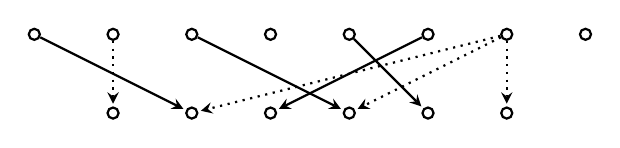
\begin{tikzpicture}[->,>=stealth,shorten >=1pt,auto,node distance=1cm, thick,main node/.style={scale=0.9,circle,draw,font=\sffamily\normalsize},
        block/.style={rectangle, draw, minimum width = 60, minimum height = 20, rounded corners = 6pt}, small circle/.style={circle, draw, inner sep=0pt, minimum size=4pt}]

            % Pigeons

            \foreach \b [
                evaluate = \b as \bprev using {int(\b-1)},
            ] in {0,1,2,3,4,5,6,7} {
                \ifnum\b=0
                  \node [small circle] (p\b) [] {};
                \else
                  \node [small circle] (p\b) [right of = p\bprev] {};
                \fi
            }

            % Holes

            \foreach \b [
                evaluate = \b as \bprev using {int(\b-1)},
            ] in {0,1,2,3,4,5} {
                \ifnum\b=0
                  \node [small circle] (h\b) [below of = p1] {};
                \else
                  \node [small circle] (h\b) [right of = h\bprev] {};
                \fi
            }

            % Pigeons

            \path[every node/.style={font=\sffamily\small}]
                  (p0) edge (h1)
                  (p1) edge[dotted] (h0)
                  (p2) edge (h3)
                  (p4) edge (h4)
                  (p5) edge (h2)
                  (p6) edge[dotted] (h1)
                  (p6) edge[dotted] (h3)
                  (p6) edge[dotted] (h5)
                ;
        \end{tikzpicture}
    }
    \caption{Graphical representation of a partial assignment on $\mathrm{PHP}^8_6$. Each edge is a variable $p_{i,j}$. Solid edges are assigned as true, missing edges are assigned as false and dotted edges are unassigned.}
    \label{fig:php}
\end{figure}

\section{Computability}

Depending on the objective, a problem can ask for a binary answer, a specific solution structure or the best possible solution out of many. We divide these problems into three categories: \textit{decision}, \textit{search} and \textit{optimization} \cite{sip_book,papad_book}. A decision problem is a problem for which we are asked to determine if a chosen property holds for a given a instance of the problem. A search problem, instead, asks to find some structure that certifies the validity of the chosen property. Similarly, an optimization problem asks us to find the optimal structure among all the available ones. It is easy to see that these three ideas form some sort of hierarchy between types of problems. In general, optimization problems are at least as hard as search problems, which in turn is at least as hard as decision problems. For $\mathsf{NP}$-complete problems (see \Cref{sec:complexity}), search and decision are generally polynomially equivalent. This property is known as \textit{self-reducibility} \cite{decision_vs_search,papad_book}.

We face these types of problems every day in our life. For instance, suppose that we want to reach a destination $B$ from a starting point $A$. If we are interested in finding the \textit{shortest} route between point $A$ and $B$, this becomes an optimization problem. If we want to find a route between the two sites, without caring about its length, this becomes a search problem. If, instead, we want to just establish the existence of at least one route, this becomes a decision problem.  

Let $\Sigma$ be a finite set of symbols (e.g. $\Sigma = \{a,b,c, 0, \$, 3, x, \ldots\}$), referred to as \textit{alphabet}, and let $\Sigma^*$ be the infinite set of all finite strings formed by characters taken from that alphabet. Any subset $L \subseteq \Sigma^*$ is referred to as a \textit{language}. Typically, we are interested in the case where $\Sigma = \{0,1\}$.

Consider a binary predicate $P : \Sigma^* \to \{0,1\}$ representing some property, meaning that $P(x) = 1$ means that the property holds for the input instance $x$ and $P(x) = 0$ means that it does not. Let $R_P \subseteq \Sigma^* \times \Sigma^*$ be the binary relation such that $R_P(x,y)$ holds if and only if $y$ certifies the fact that $P(x) = 1$. We refer to $\mathrm{Sol}_P(x) = \{y \in \Sigma^* \mid R_P(x,y)\}$ as the set of \textit{solutions} (or \textit{witnesses}) for the instance $x$ over the property $P$.

\begin{definition}
  The decision problem of $P$ is defined as the language $\Pi_{\text{dec}}^P = \{x \in \Sigma^* \mid \mathrm{Sol}_P(x) \neq \varnothing\}$. The problem $\Pi_{\text{dec}}^P$ is said to be decidable (or computable) if there is an algorithm $\mathcal{A}$ such that $\mathcal{A}(x) = 1$ when $\mathrm{Sol}_P(x) \neq \varnothing$ and $\mathcal{A}(x) = 0$ otherwise.
\end{definition}

We observe that the above definition of computability for decision problem can also be stated as the existence of an always-halting algorithm $L(\mathcal{A}) =\Pi_{\text{dec}}^P$. Moreover, we also observe that the above definition could've been stated without the use of the binary relation $R_P$ since $\Pi_{\text{dec}}^P = \{x \in \Sigma^* \mid P(x) = 1\}$ is an equivalent definition. In this setting, the definition is given using $R_P$ only for consistency with search and optimization problems. In fact, for the other two types of problems binary relations are necessary due to the fact that one instance may have more than one possible witness. For instance, there may be more than one (optimal) route from point $A$ to point $B$.

\begin{definition}
  The search problem of $P$ is defined as the binary relation $\Pi_{\text{search}}^P = R_P$. The problem $\Pi_{\text{search}}^P$ is said to be solvable (or computable) if there is an algorithm $\mathcal{A}$ such that $\mathcal{A}(x) \in \mathrm{Sol}_P(x)$ when $\mathrm{Sol}_P(x) \neq \varnothing$ and $\mathcal{A}(x) = \bot$ otherwise.
\end{definition}

Here, the symbol $\bot$ is used to represent the fact that no solution exists for the given input instance. The definition allows any algorithm computing the problem to return a different solution on each execution. Optimization problems require an additional component: a \textit{cost function} $c : \Sigma^* \times \Sigma^* \to \R$ expressing the optimality of the solution for the given instance. We denote the set of optimal solutions as $\mathrm{Opt}_P(x) = \{y \in \mathrm{Sol}_P(x) \mid c(x,y) = \max_{z \in \mathrm{Sol}_P(x)} c(x,z)\}$. Notice that each maximization problem can be rewritten as an equivalent minimization problem. 

\begin{definition}
  The optimization problem of $P$ over $c$ is defined as the binary relation $\Pi_{\text{opt}}^P = \{(x,y) \in \Sigma^* \times \Sigma^* \mid y \in \mathrm{Opt}_P(x)\}$. The problem $\Pi_{\text{opt}}^P$ is said to be solvable (or computable) if there is an algorithm $\mathcal{A}$ such that $\mathcal{A}(x) \in \mathrm{Opt}_P(x)$ when $\mathrm{Sol}_P(x) \neq \varnothing$ and $\mathcal{A}(x) = \bot$ otherwise.
\end{definition}

As previously stated, these three categories form a hierarchy of problems. This is clear from their own definitions: any algorithm computing an optimization problem also computes a search problem and any algorithm computing a search problem can be adapted into one that computes a decision problem.

\section{Computational complexity}
\label{sec:complexity}
In his seminal work, Turing \cite{turing} proved that some problems are \textit{undecidable}, meaning that there is no algorithm that can compute them exactly. Following his work, the pioneers of computer science started noticing that even though many problems can be computed, the algorithms computing them would take too many resources, making them infeasible to process for large inputs. In particular, they focused on two main measures: \textit{time} and \textit{space} \cite{complexity_measures,sip_book,arora_barak}. 

\begin{definition}
  Let $\mathcal{A}$ be an algorithm and let $t, s \colon \N \to \R^+$ be two functions. We say that $\mathcal{A}$ \emph{runs in time} $t$ if on every input $x$ the algorithm halts after at most $t(|x|)$ steps and that $\mathcal{A}$ \emph{runs in space}
  $s$ if on every input $x$ it uses at most $s(|x|)$ memory cells.
\end{definition}

These two complexity measures are intrinsically related one to another and they are, usually, negatively correlated. Generally, if we allow our algorithm to use more space then the computation can be sped up by saving partial computations, while if we want to lower the amount of space needed then these partial computations have to be calculated each time they are required. Larger inputs require larger amounts of computational resources, making the values $t(n)$ and $s(n)$ proportional to the size $n$ of the input.

Usually, we work with these measures as the input length grows asymptotically. In particular, borrowing notation from standard calculus, we are interested in bounding costs from above and below, up to some constant factor. Let $f,g : \N \to \R^+$ be two functions. We say that:
  \begin{itemize}[nosep]
    \item $f(x)$ is in $O(g(x))$ when there are two constants $c,n_0 > 0$ such that $\forall n \geq n_0$ we have $f(n) \leq c \cdot g(n)$;
    \item $f(x)$ is in $\Omega(g(x))$ when there are two constants $c,n_0 > 0$ such that $\forall n \geq n_0$ we have $f(n) \geq c \cdot g(n)$;
    \item $f(x)$ is in $\Theta(g(x))$ when $f(x)$ is both in $O(g(x))$ and $\Omega(g(x))$;
    \item $f(x)$ is in $o(g(x))$ when for each constant $c > 0$ there is a constant $n_0 > 0$ such that $\forall n \geq n_0$ we have $f(n) < c \cdot g(n)$.
  \end{itemize}

The main goal of computational complexity is establishing what can and cannot be solved under some complexity measure constraints. In real world situations, any algorithm with runtime larger than $O(n^3)$ is considered impractical since it requires too much time for large inputs. Nonetheless, complexity theorists use this to their advantage: if a problem cannot be solved even when allowing this constraint to be any form of \textit{polynomial time}, i.e. time $O(n^c)$ for some $c > 0$, the problem is ruled out as \textit{intractable}. Therefore, in this context efficient and polynomial-time are considered synonyms of each other. The class of all efficiently solvable decision problems is denoted with $\mathsf{P}$ and the same holds for $\mathsf{FP}$, the class of efficiently solvable search problems \cite{cobham_p,arora_barak}.

\begin{definition}
  We define $\mathsf{P}$ as the class of decision problems solvable in polynomial time by an algorithm, i.e. in time $O(n^c)$ for some $c > 0$. Similarly, $\mathsf{FP}$ is the class of search problems solvable in polynomial time.
\end{definition}

The aforementioned $\mathsf{P}$ vs. $\mathsf{NP}$ question (or $\mathsf{FP}$ vs. $\mathsf{FNP}$ for search problems) asks to settle if the class of efficiently solvable problems corresponds to the class of efficiently verifiable problems. Here, a \textit{verifier} for a problem $L$ is an algorithm that takes an additional input $w$, referred to as the \textit{witness}, and uses it to check if $x \in L$ holds or not. Usually, this witness is a string that describes a real solution of the problem for the given input. The length of the witness must be bounded by at most a polynomial with respect to the input length.

\begin{definition}
  We define $\mathsf{NP}$ as the class of decision problems verifiable in polynomial time by a verifier. In particular, for an $\mathsf{NP}$ language with verifier $V$, it holds that $x \in L$ if and only if $\exists w \in \Sigma^*$ for which $V(x,w) = 1$ and $\abs{w} \leq O(\abs{x}^c)$ for some $c > 0$.
\end{definition}

By definition, we have that $\mathsf{P} \subseteq \mathsf{NP}$ since if a problem is efficiently solvable then we can just ignore the given witness and solve the problem. Hence, the $\mathsf{P}$ vs. $\mathsf{NP}$ question asks to settle if this inclusion also holds in the converse direction, i.e.  $\mathsf{NP} \subseteq \mathsf{P}$. After more than 50 years of scientific literature studying this problem and its ramifications, researchers conjecture that the answer to this problem is negative \cite{sipser_pnp,arora_barak, aaronson_survey}.

\begin{conjecture}
  $\mathsf{P} \neq \mathsf{NP}$
\end{conjecture}

For our purposes, we will assume this conjecture to be true. Another class of our interest is the class $\mathsf{coNP}$, defined as the set of all problems whose complement is verifiable in polynomial time.

\begin{definition}
  $\mathsf{coNP} = \{L \subseteq \Sigma^* \mid \overline{L} \in \mathsf{NP}\}$.
\end{definition}

it is easy to see that problems that lie in $\mathsf{coNP}$ admit a verifier that uses witnesses to discard invalid input instances: if $w$ is a witness for the membership of $x$ in $\overline{L}$ then $w$ is also a witness for the non-membership of $x$ in $L$. In other words, a problem is in $\mathsf{NP}$ if its correct instances can be efficiently verified, while a problem is in $\mathsf{coNP}$ if the same holds for incorrect instances. 

Again, it is easy to see that $\mathsf{P} \subseteq \mathsf{coNP}$, but the converse is not known and it is actually a question equivalent to establishing that $\mathsf{P} = \mathsf{NP}$. This is due to the fact that if a problem is efficiently solvable then its complement is also efficiently solvable (we can just negate the output of the same algorithm). This same reasoning implies that if $\mathsf{P} = \mathsf{NP}$ then $\mathsf{NP} = \mathsf{coNP}$. Therefore, proving that $\mathsf{NP} \neq \mathsf{coNP}$ could be a way of establishing that $\mathsf{P} \neq \mathsf{NP}$. It is also conjectured that $\mathsf{NP} \neq \mathsf{coNP}$: there are evident asymmetries between the hardness of witnessing that something holds and that of witnessing something does not hold both in mathematics and computer science \cite{cook_proof_compx}.

\begin{conjecture}
  $\mathsf{NP} \neq \mathsf{coNP}$
\end{conjecture}

Going upwards with time complexity, we will also be interested in the quasi-polynomial and sub-exponential analogues of $\mathsf{P}$, referred to as the classes $\mathsf{QP}$ and $\mathrm{SUBEXP}$ \cite{arora_barak}, respectively. Here, \textit{quasi-polynomial} means that the runtime is a polynomial with at most a poly-logarithmic exponent, while \textit{sub-exponential} means any runtime that is strictly inferior to exponential time.

\begin{definition}
  We define $\mathsf{QP}$ as the class of decision problems solvable in quasi-polynomial time by an algorithm, i.e. in time $O(n^{\log^c n})$ for some $c > 0$. Similarly, $\mathsf{SUBEXP}$ is the class of decision problems solvable in less than exponential time, i.e. in time $O(2^{n^\varepsilon})$ for all $\varepsilon > 0$.
\end{definition}

By definition, we have that $\mathsf{P} \subseteq \mathsf{QP} \subseteq \mathsf{SUBEXP}$. No relationship between $\mathsf{NP}$ and $\mathsf{QP}$ or $\mathsf{SUBEXP}$ is known. However, both $\mathsf{NP} \subseteq \mathsf{QP}$ and $\mathsf{NP} \subseteq \mathsf{SUBEXP}$ are conjectured to be false. Since the decision problems underlying most cryptographic assumptions lie in $\mathsf{NP} \cap \mathsf{coNP}$, if $\mathsf{NP} \subseteq \mathsf{QP}$ were to be true then all such assumptions would be breakable in quasi-polynomial time, which is believed to be false. $\mathsf{NP} \subseteq \mathsf{SUBEXP}$ is also conjectured to be false, mainly due to the \textit{Exponential Time Hypothesis} (see \Cref{sec:auto_treelike}).

\begin{conjecture}
  $\mathsf{NP} \not\subseteq \mathsf{QP}$ and $\mathsf{NP} \not\subseteq \mathsf{SUBEXP}$.
\end{conjecture}

Finally, we define one last class that introduces randomized computation \cite{gill_zpp}. Intuitively, a randomized algorithm is an algorithm that is allowed to generate random bits according to a probability distribution, typically set to the uniform distribution over $0$ and $1$. In this work we will be interested in only one particular type of randomized computation, referred to as \textit{zero-sided error computation}. A randomized algorithm is said to have zero-sided error when for each generable sequence of randomized bits the algorithm never makes mistakes, but it is allowed to answer with \curlyquotes{I do not know} with probability at most $1/2$. The class of problems efficiently solvable by these algorithms is referred to as $\mathsf{ZPP}$. We observe that $\mathsf{P} \subseteq \mathsf{ZPP} \subseteq \mathsf{NP} \cap \mathsf{coNP}$.

\begin{definition}
  We define $\mathsf{ZPP}$ as the class of decision problems solvable in polynomial time by a zero-sided error algorithm, i.e. in time $O(n^c)$ for some $c > 0$.
\end{definition}

To interact with these classes we often use the concept of reductions between problems \cite{karp,sip_book}. The idea of problem reduction is simple: if there is a reducing function between an initial problem $A$ and a target problem $B$ and $B$ can be solved then $A$ can also be solved by using the reduction as a tunnel. This is due to the fact that if an algorithm for the original problem can simply compute the reduction and then execute the algorithm that solves the new problem.

\begin{definition}[Many-to-one reduction]
  Let $A$ and $B$ be two decision problems. We say that $A$ many-to-one reduces to $B$, written as $A \leq_m B$ when there is a computable function $f : \Sigma^* \to \Sigma^*$ such that $x \in A$ if and only if $f(x) \in B$. 
\end{definition}

When $A \leq_m B$ holds, we say that $B$ is \curlyquotes{at least as hard as} $A$ since solving $B$ implies solving $A$. If the reduction is computable in polynomial time, we say that $A$ \textit{p-reduces} to $B$, written as $A \leq_p B$. In two seminal papers, Cook and Levin \cite{cook_sat,levin_fsat} independently showed that the \textit{satisfiability problem} $\mathrm{SAT} = \{\abk{\varphi} \mid \varphi \text{ a satisfiable CNF}\}$, where $\abk{\cdot}$ denotes binary encoding, is $\mathsf{NP}$-hard, meaning that every problem that lies in $\mathsf{NP}$ is many-to-one reducible to it. Under the assumption that $\mathsf{P} \neq \mathsf{NP}$, this makes this problem unsolvable in polynomial time.

\section{Decision trees}

\textit{Decision trees} are a simple computational model used in many areas of computer science \cite{jukna,arora_barak}. In our case, we will consider decision trees as a way to compute Boolean functions $f : \{0,1\}^n \to \{0,1\}$ or, more generally, for search problems based on such functions. Informally, decision trees are graphical representations of algorithms for computing a function of an unknown input. Each node of the tree is labeled by a variable $x_i$, $i \in [n]$, and the branches from that node are labeled by the possible values of the variable ($0$ or $1$ in our case). The leaves are labeled by the output of the function. The process starts at the root, knowing nothing, works down the tree, choosing to learn the values of some of the variables based on those already known and eventually reaches a decision.

\begin{definition}
 A decision tree is a rooted directed binary tree whose nodes are associated with either an output value or an input Boolean variable. Each internal node is labeled by a variable and the two outgoing edges are labeled by the two possible values. Each leaf is labeled with an output $o \in O$, for a set of outputs $O$.
\end{definition}

A Boolean function $f$ is said to be computed by a decision tree $\mathcal{T}$ when for each input $x$ it holds that $f(x) = \mathcal{T}(x)$. For this computation model we are interested in two main complexity measures: depth and size \cite{jukna, dt_survey}. The \textit{depth} of a decision tree is the number of edges in a longest path from the root to a leaf, or equivalently, the maximum number of bits tested on such a path. The \textit{size} of a decision tree, instead, is the number of nodes in the tree. Generally, for a Boolean function $f$ we denote with $D(f)$ the minimum depth across all decision trees computing $f$.

An interesting property of decision trees is their possibility to be represented as propositional formulas. In particular, a depth-$d$ decision tree $\mathcal{T}$ computing $f$ gives rise to both a $d$-DNF and a $d$-CNF representation for $f$.

Let $\mathrm{Leaves}(\mathcal{T})$ be the set of all leaves in $\mathcal{T}$ and let $\mathrm{out}(\ell)$ be the output value associated with a leaf $\ell \in \mathcal{T}$. Then, the associated $d$-DNF $\mathrm{DNF}(\mathcal{T})$ is given by

\begin{equation}
  \mathrm{DNF}(\mathcal{T}) := \bigvee_{\substack{\ell \in \mathrm{Leaves}(\mathcal{T}) :\\ \mathrm{out}(\ell) = 1}} D_\ell
\end{equation}

\noindent
where $D_\ell$ is the conjunction of all the literals corresponding to the query outcomes on the path from the root of $\mathcal{T}$ to the leaf $\ell$. If the query $x_i$ has outcome 1, the corresponding literal is $x_i$, otherwise it is $\lnot x_i$. The associated $d$-CNF, instead, is obtained by negating the $d$-DNF formula associated with the negated decision tree $\lnot \mathcal{T}$, corresponding to the tree $\mathcal{T}$ with inverted output values, computing $\lnot f$. For instance, the decision tree shown in \Cref{fig:decision_tree} can be represented as the DNF formula
\begin{equation}
  (\lnot x_1 \land x_2 \land \lnot x_3) \lor (\lnot x_1 \land x_2 \land x_3) \lor (x_1 \land \lnot x_3 \land x_2)
\end{equation}
\noindent
or as the CNF formula obtained by negating the DNF of the inverted tree
\begin{equation}
  (x_1 \lor x_2 \lor x_3) \land (x_1 \lor x_2 \lor \lnot x_3) \land (\lnot x_1 \lor x_3 \lor x_2) \land (\lnot x_1 \lor \lnot x_3)
\end{equation}

\begin{figure}[t]
    \centering

    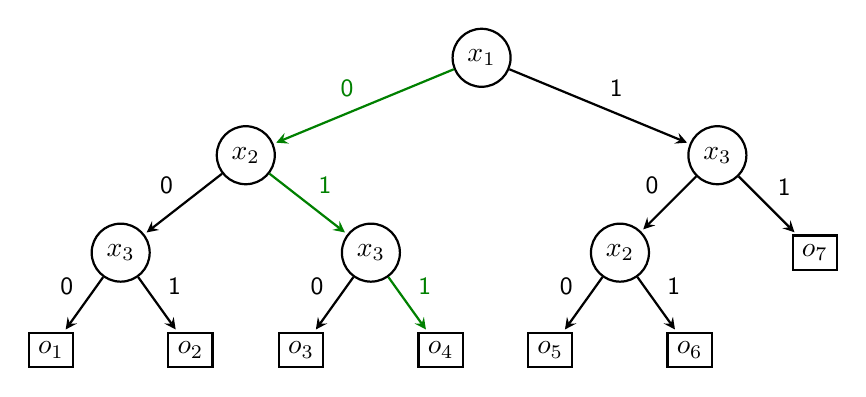
\begin{tikzpicture}[->,>=stealth,shorten >=1pt,auto,node distance=1.75cm, thick,main node/.style={scale=0.9,circle,draw,font=\sffamily\normalsize}]

        \node[circle, draw] (1)[] {$x_1$};

        \node[circle, draw] (2) [below left of=1, xshift=-50, ]{$x_2$};
        \node[circle, draw] (3) [below right of=1, xshift=50, ]{$x_3$};

        \node[circle, draw] (4) [below left of=2, xshift=-10, ]{$x_3$};
        \node[circle, draw] (5) [below right of=2, xshift=10, ]{$x_3$};
        \node[circle, draw] (6) [below left of=3, ]{$x_2$};
        \node[rectangle, draw] (7) [below right of=3]{$o_7$};

        \node[rectangle, draw] (8) [below left of=4, xshift=10]{$o_1$};
        \node[rectangle, draw] (9) [below right of=4, xshift=-10]{$o_2$};
        \node[rectangle, draw] (10) [below left of=5, xshift=10]{$o_3$};
        \node[rectangle, draw] (11) [below right of=5, xshift=-10]{$o_4$};
        \node[rectangle, draw] (12) [below left of=6, xshift=10]{$o_5$};
        \node[rectangle, draw] (13) [below right of=6, xshift=-10]{$o_6$};

        \path[every node/.style={font=\sffamily\small}]
        (1) edge[swap, color=Green]  node{0} (2)
        (1) edge node{1}(3)

        (2) edge[swap]  node{0} (4)
        (2) edge[color=Green]  node{1}(5)

        (3) edge[swap]  node{0} (6)
        (3) edge  node{1}(7)
                    
        (4) edge[swap]  node{0} (8)
        (4) edge  node{1}(9)

        (5) edge[swap]  node{0} (10)
        (5) edge[color=Green]  node{1}(11)

        (6) edge[swap]  node{0} (12)
        (6) edge  node{1}(13)
        ;
    \end{tikzpicture}

    \caption{An example of a decision tree of size 13 and depth 3. The green path shows the computation made for the input $x = 011$.}
    \label{fig:decision_tree}
\end{figure}

\cleardoublepage